\documentclass[10pt,conference,compsocconf]{IEEEtran}
\usepackage{tikz}
\usepackage{pgf}
\usepackage{pgfplots}
\usetikzlibrary{arrows,automata}

\begin{document}

  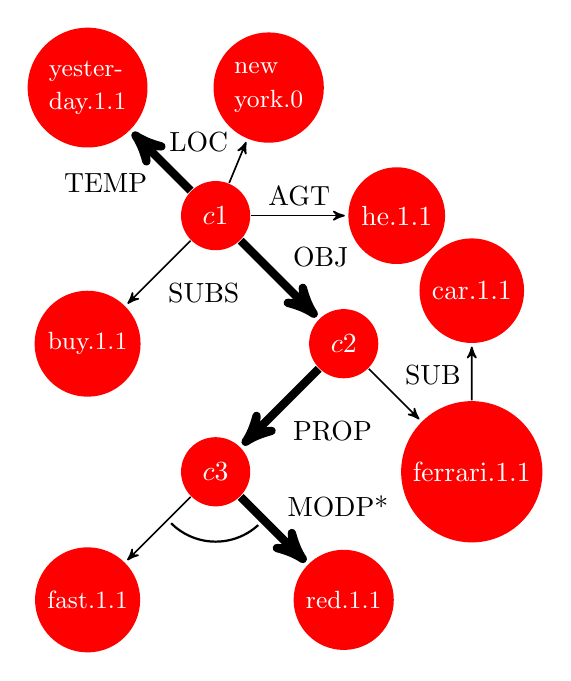
\begin{tikzpicture}[>=stealth',shorten >=1pt,auto,node distance=2.3cm,
                    semithick,scale=0.1]
  \tikzstyle{every state}=[fill=red,draw=none,text=white]

  \node[state] (A)                    {$c1$};
 \node[state]         (B) [right of=A] {he.1.1}; %below left of=
  \node[state]         (P) [below right of=A] {$c2$};
  \node[state]         (E) [below left of=A] {\small buy.1.1};
  \node[state]         (C) [below left of=P]       {$c3$};
  \node[state]         (D) [below right of=P]   {ferrari.1.1} ;
  \node[state]         (F) [below left of=C]  {\small fast.1.1};
  \node[state]         (G) [below right of=C] {\small red.1.1} ;
  \node[state]         (H) [above left of=A] {$c4$};
  \node[state,align=left]         (I) [right of=H]{\small new\\\small york.0};
  \node[state,align=left]         (J) [above left of=A] {\small yester-\\\small day.1.1};
  \node[state]         (K) [above of=D] {car.1.1};


\draw [->] (A) edge node {AGT} (B);
\draw [->] (A) edge node {SUBS} (E);
\draw [->, line width=3pt] (A) edge node {OBJ} (P);
\draw [->] (A) edge node {LOC} (I);
\draw [->,line width=3pt] (A) edge node {TEMP} (J);
\draw [->, line width=3pt] (P) edge node {PROP} (C);
\draw [->] (P) edge node {SUB} (D);
\draw [->] (D) edge node {} (K); 
\draw [->, line width=3pt] (C) edge node {MODP*} (G);
\draw [->] (C) edge node {} (F);

\draw [thick,domain=225:315] plot ({8*cos(\x)}, {-33.4+8*sin(\x)});
\draw (0.8,-9.4) -- (1,-9.1);
\draw (0.7,-9.15) -- (1,-9.15);


\end{tikzpicture}

\end{document}